\chapter{Verwendete Methodiken}
\label{chap_Body}
Nach der Einführung zu den verschieden Themenbereichen, nun zu den eigentlichen Methodiken, welche entweder schon vorhanden sind, oder im Zuge dieser Arbeit erarbeitet wurden.
\section{Ladeservice und Ladeprozess}
Ein Ladeservice startet, wenn ein Elektrofahrzeug mit einem passenden Ladegerät verbunden wird und endet, wenn eben diese Verbindung wieder getrennt wird. Während dieser Zeit soll sich der Ladezustand des Fahrzeuges entweder auf 100~\% erhöhen, oder wenn dies, aufgrund von zeitlichen oder technischen Limitierungen nicht möglich ist, möglichst nah an 100~\% annähern. Die Qualität des Ladeservices hängt vom Ladezustand des Elektrofahrzeuges bei Beendigung des Ladeservices ab. Je geringer der Abstand zu einem Ladezustand von 100~\% desto höher ist die Qualität eines Ladeservice. Die Erhöhung des Ladezustands geschieht durch Ladevorgänge. Ein Ladeservice kann mehrere Ladevorgänge beinhalten. Die bloße Anzahl von Ladevorgängen in einem Ladeservice mindert potenziell nicht die Qualität des Services. Ein Ladevorgang erhöht den Ladezustand der Batterie durch Verwendung von elektrischer Energie, welche aus dem Netz bezogen wird. Ein Ladevorgang ist zeitlich unbeschränkt und endet wegen technischen Limitierungen oder wenn der Ladeservice, welcher den Ladevorgang enthält, endet. Technische Limitierung welche das Ende eines Ladeprozesses verursachen sind das nicht einhalten von Schwellenwerten in Hinsicht auf Spannung, Ladezustand des Fahrzeuges und Belastungen im Stromnetz. Im Ladevorgang selbst werden Geräte verwendet, welche elektrischen Strom benötigen, wenn dieser Strom nicht bei ausreichender Spannung vorliegt, muss der Ladevorgang abgebrochen werden. Ein Elektrofahrzeug kann keinen Ladezustand von mehr als 100~\% aufweisen, werden bei einem Ladevorgang 100~\% Ladezustand erreicht werden, endet der Ladevorgang. Bei einer zu hohen Belastung am Stromnetz wird im Sinne der Materialschonung der Ladevorgang beendet. Die Beendigung eines Ladevorgangs ist nicht gleichzusetzen mit dem Ende des Ladeservice an sich. 
\begin{figure}[tb]
	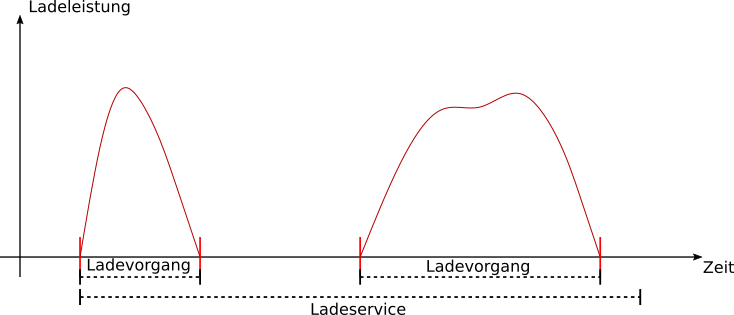
\includegraphics[width=\linewidth]{img/Ladeservice.png}
	\caption{Verlauf eines Ladeservices}
	\label{Abb_Ladeservice}
\end{figure}

In der Abbildung \ref{Abb_Ladeservice} wird die Aktivität innerhalb eines Ladeservices aufgezeigt. Der dargestellte Ladeservice enthält zwei Ladevorgänge. Die Länge beider Ladevorgänge zusammen ist kürzer als die Länge des Ladeservices.\\
Der Wert der Qualitätserfahrung der Ladeservices wird mithilfe der Hoßfeld Methode \cite{Hosfeld2018} berechnet. Diese Methode bezieht die Standardabweichung vom Ergebnis als auch die maximal und minimal möglichen Werte des Ergebnisses mit ein. Der Wert der Fairness wird mit folgender Formel F($\sigma$) berechnet.
\begin{align}
	F(\sigma) = 1-\frac{2*\sigma}{100}
\end{align}
$\sigma$ steht für die Standardabweichung des Ladezustandes beim Verlassen der Ladestation. Die 100 im Nenner des Bruches kommt zustande durch die Subtraktion des niedrigsten möglichen Wertes vom höchst möglichen Wert, 100 – 0. Das Ergebnis der Formel liegt im Bereich von 1 bis 0, (0,1). Je höher das Ergebnis der Formel, desto höher ist die Qualitätserfahrung zwischen den Teilnehmern. Die zu Beginn niedrigere Fairness lässt sich auf die zu Beginn auch hohe Standardabweichung beim Ladestand der einzelnen Fahrzeuge zurückführen. Je geringer die Standardabweichung allerdings wird, desto höher steigt auch der Wert der Qualitätserfahrung. Vergleicht man die Qualitätserfahrungen der Teilnehmer miteinander, ergibt sich ein Qualitätserfahrungs Fairness Index.
\section{Datengrundlage}
\label{cap:background_sec:setting}
Während eines Ladeservices kann für die Beurteilung der aktuellen Situation auf verschiedene Daten zugegriffen werden. Es ist die Ankunftszeit, also der Beginn des Ladeservices, bekannt, ebenso wie die Abfahrtszeit, welche das Ende des Ladeservices markiert. Neben der Anfangs- und Endzeit, ist auch der aktuelle Zeitpunkt bekannt. Die aktuelle Zeit erhöht sich periodisch um immer den selben Wert und kann so in diskrete Zeiteinheiten eingeteilt werden. Des weiteren ist in jedem Zeitpunkt des Ladeservices der Ladezustand des Fahrzeuges, die aktuelle Spannung am Anschlusspunkt und die maximale nutzbare Stromstärke des Fahrzeuges des jeweiligen Teilnehmers bekannt. Über ein Broadcastsystem wird innerhalb eines Anschlussbereiches von jedem Teilnehmer, welcher aktuell einen Ladeservice durchführt, die Information das ein solcher Prozess stattfindet verteilt. Über das selbe Broadcastsystem wird von den Transformatoren des Anschlussbereiches die aktuelle Menge an Scheinleistung, welche in den Anschlussbereich abgegeben wird verteilt. Durch Sammlung der Meldungen von Fahrzeugen, welche gerade einen Ladeservice durchführen, lässt sich die Anzahl der aktuell stattfindenden Ladeservices im Anschlussbereich ermitteln. Der Anschlussbereich in dem diese Daten verbreitet werden umfasst jeweils ein einzelnes Niederspannungsnetz.  Es wird in dieser Arbeit im Folgenden davon ausgegangen, das das verwendete Broadcastsystem keinen nennenswerten Delay aufweist und eine hohe Verfügbarkeit hat. Somit wird davon ausgegangen, dass die Daten immer übertragen werden und so immer verwendet werden können.

\section{Spannungsregler nach VDE 4100}
\label{capBody:VDE}
Die erste Methodik dient als Grundlinie für den Vergleich der später folgenden Methodiken. Diese Methodik stellt die aktuell im Stromnetz vorliegende Situation dar. Sie verwendet die technische Anschlussregel Niederspannung (VDE-AR-N 4100), diese stellt neue Anforderungen an die Ladegeräte von Elektrofahrzeugen. Sie wurde ebenfalls entwickelt, um eine größere Anzahl von Ladegeräten am Netz nutzbar zu machen \cite{kutter2020}. Bei der verwendeten Form der Anschlussregel, handelt es sich um einen Spannungsregulator, welcher anhand der Spannung angibt, wie viel der aktuell möglichen Leistung abgerufen wird. Bei einem gemessenen Wert der Spannung von mehr als 93~\% der Normspannung, kann die Leistung wie gefordert abgerufen werden. Ab einer Spannung von weniger als 88~\% der Normspannung kann keine Leistung mehr angerufen werden. In dem Bereich von 93~\% bis 88~\% der Normspannung wird die abrufbare Leistung linear reduziert, von voller hin zu keiner abrufbaren Leistung.

\begin{figure}[htb]
	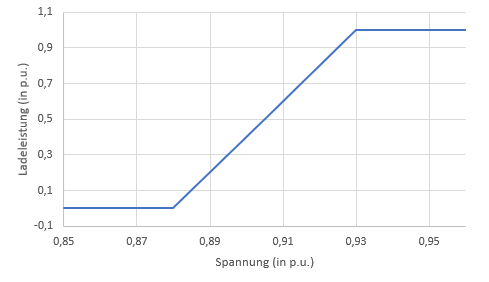
\includegraphics[width=\linewidth]{img/VDE3.png}
	\caption{Spannungs zu Leistungsverhältnis nach VDE-AR-N 4100}
	\label{Abb_VDEController}
\end{figure}

Der Graph in Abbildung \ref{Abb_VDEController} zeigt die mögliche Ladeleistung bei dem prozentualen Anteil der Normspannung. Auf der Y-Achse ist die mögliche Ladeleistung angetragen, wobei eins für die höchstmögliche Leistung steht und null dafür, dass für keine Leistung abrufbar ist. An der X-Achse werden die aktuell anliegenden Prozent der Normspannung angetragen. An dem Graphen ist ersichtlich, dass bei mehr als 93~\% der Normspannung die ganze Ladeleistung zur Verfügung steht. Es ist weiterhin erkennbar, wie sich die mögliche Ladeleistung im Bereich von 93~\% bis 88~\% der Normspannung verhält. Ebenso ist erkennbar, wie das keine Ladeleistung bei einem Wert von weniger als 88~\% der Normspannung mehr möglich ist. \\
Die Ladeleistung P\textsubscript{L} wird berechnet mithilfe der aktuellen Spannung U\textsubscript{A} und der aktuell maximal nutzbaren Stromstärke I\textsubscript{F} des Fahrzeuges durch die Formel
\begin{align}
	P\textsubscript{L} = U\textsubscript{A} \cdot I\textsubscript{F} \label{Main_formula1}
\end{align}
Bei der Formel \ref{Main_formula1} wird von einer Spannung von über 93~\% der Normspannung ausgegangen, da die berechnete Ladeleistung nicht verändert wird. Im Bereich von unter 93~\% der Normspannung ist eine solche Änderung aber nötig. Der Faktor F, mit dem der verbliebene Anteil der möglichen Ladeleistung berechnet wird, wird wie folgt bestimmt \\
\begin{center}
	$ F = \begin{cases}
	1 &  \text{$>$ 93\% Normspannung} \\
	0 &  \text{$<$ 88\% Normspannung} \\
	20 \cdot \frac{U\textsubscript{A}}{U\textsubscript{N}} - 17.6 & \text{$>$ 88\%, $<$ 93\% Normspannung}
	\end{cases}
	$
\end{center}
Der Wertebereich der Formel ist bei Null bzw. Eins abgeschlossen. Bei zu niedrigen Spannungswerten, weniger als 88\% der Normspannung, wird der Faktor ohne Berechnung der Formel mit Null angegeben. Ergebnisse größer als Eins werden auf eins reduziert, da alle Werte größer als Eins in einer höheren Ladeleistung als überhaupt möglich resultieren würden. \\
Wird nun der Faktor F in Formel \ref{Main_formula1} berücksichtigt, ergibt sich folgende Formel für die mögliche Ladeleistung\\
\begin{align}
	P\textsubscript{L} = U\textsubscript{A} \cdot I\textsubscript{F} \cdot F \label{Main_formula3}
\end{align}
Bevor die mithilfe des VDE-AR-N 4100 Spannungsregler bestimmte mögliche Ladeleistung tatsächlich bezogen wird, wird bei dieser Methodik der Wert zuerst gefiltert. Diese Filterung erfolgt mit Hilfe eine First-Order Lag Filters. Bei einem First-Order Lag Filter wird eine Änderung zwischen dem aktuellen und einem neu berechneten Wert nicht komplett vollzogen, sondern nur teilweise. Ein solcher Filter dient der Dämpfung von oszillierenden Signalen hin zu einem homogenerem Verlauf . In der hier verwendeten Form werden nur 63,2~\% der eigentlichen Änderung vorgenommen. So steigen Werte nur um 63,2~\% der eigentlichen Steigerung, ebenso fallen Werte nur um 63,2~\% der Änderung. Der Wert von 63,2~\% wurde gewählt um in nur wenigen Schritten eine möglichst nahe Annäherung an den eigentlich Wert zu erreichen.
\begin{figure}[htb]
	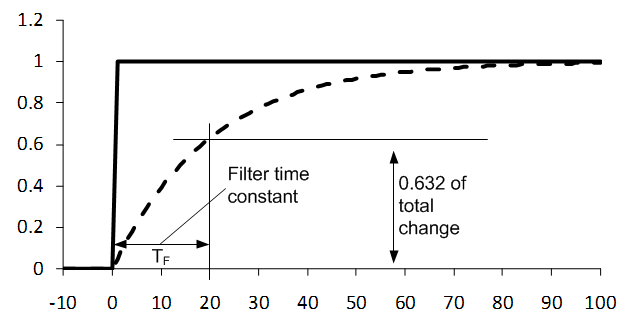
\includegraphics[scale=0.75]{img/lag_Filter.png}
	\caption{Wirkung eines First-Order Lag Filters beim Wechsel des \newline Eingangsignals von Null auf Eins}
	\label{Abb_lag_filter}
\end{figure}

Aus der Abbildung \ref{Abb_lag_filter} wird ersichtlich, wie ein First-Order Lag Filter auf ein starkes Wachstum eines Wertes reagiert. Die durchgezogene Linie, welche beim Zeitpunkt null auf einen Wert von eins steigt, zeigt den Verlauf ohne Filter. Die gestrichelte Linie, welche im Zeitpunkt null beginnt, zeigt den Verlauf mit Filter. T\textsubscript{F} zeigt die Dauer des verwendeten Zeitintervalls. Die schwarzen Linien, beginnend bei einem Wert von zwanzig auf der X-Achse, markieren an ihrem Schnittpunkt  mit der gestrichelten Linie den Wert nach der ersten Anwendung des Filters. Dieser Wert liegt bei 63,2\% der eigentlichen Änderung. Bei fortlaufender Zeit nähert sich die gestrichelte Linie der durchgezogen Linie immer weiter an.

\section{Slotted ALOHA Spannungsregler mit Fokus auf Fairness}
Bei den nächsten vorgestellten Methoden wurden Bestandteile des Slotted Aloha Protokolls (Kapitel \ref{capBack:Aloha}) verwendet. Das Slotted Aloha Protokoll arbeitet auf einem geteilten Medium, welches von allen Teilnehmern verwendet wird. Dieses geteilte Medium ist in diesem Fall das in Kapitel \ref{capBack:Stromnetz} vorgestellte Niederspannungsnetz mit den dazugehörigen elektrischen Leitern und dem verbautem Transformator. Die elektrischen Leiter im Niederspannungsnetz bedienen jeweils mehr als einen Anschluss, stehen also mehr als einem Teilnehmer gleichzeitig zur Verfügung. Der Transformator wird ebenfalls von mehr als einem Teilnehmer verwendet. Diese Teilung lässt sich auf seine einzigartige Schlüsselrolle, der Bereitstellung elektrischer Energie, und die Tatsache, dass alle Leiter mit ihm verbunden sind, zurückführen.\\
\begin{figure}[htb]
	\centering
	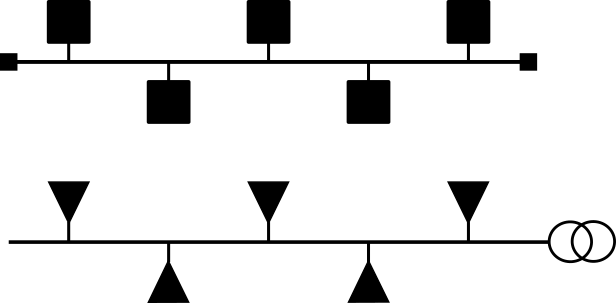
\includegraphics[scale=0.75]{img/sharedMedium3.png}
	\caption{Vergleich von Aloha Netzwerkprotokoll und Stromnetz}
	\label{Abb_sharedmedium}
\end{figure}
In der Abbildung \ref{Abb_sharedmedium} ist in der oberen Hälfte ein möglicher Aufbau eines Netzes zu sehen, in dem man das Aloha Netzwerkprotokoll, sowohl in der herkömmlichen aber auch in der slotted Variante, verwenden könnte. Die fünf, größeren Kästchen stellen die Teilnehmer dar, die beiden kleineren markieren die Grenzen des Netzes. Die Linien stehen für das eigentliche geteilte Medium. Im unteren Teil des Bildes ist ein möglicher Aufbau eines Niederspannungsnetzes mit einem Transformator und fünf Teilnehmern dargestellt. Das dargestellte Niederspannungsnetz verfügt über nur einen Strahl. Der Transformator wird durch das Kästchen dargestellt, zwei ineinander verschobene Kreise stellen jeweils einen Teilnehmer dar. Die ersichtlichen Ähnlichkeiten der physischen Aufbauten lässt erneut den Schluss zu das sich das geteilte Medium im Fall des Aloha Netzwerkprotokolls und im Fall des Stromnetzes vergleichen lässt.\\
Im Aloha Netzwerkprotokoll werden Informationen mithilfe von Frames transportiert. Im Stromnetz werden elektrische Teilchen über elektrische Leitung transportiert. Ein Frame hat allerdings eine zuvor festgelegte Größe, welche nicht unter- oder überschritten werden darf. Leistung kann über einen beliebigen Zeitraum in jeder technisch machbaren Höhe bezogen werden. Teilt man die Zeit allerdings in diskrete Abschnitte ein, so ergibt sich eine maximale Menge an Leistung, welche in diesem Zeitraum bezogen werden kann. Sollte kein ganzer Zeitslot benötigt werden, gibt es jedoch auch eine Lösung. Im Falle des Aloha Netzwerkprotokolls gibt es die Möglichkeit einen Frame, welcher nicht vollständig mit Daten gefüllt werden kann, mit Fülldaten zu ergänzen, um einen vollständigen Frame zu erhalten. Im Stromnetz wird durch einen niedrigeren Leistungsbezug als eigentlich möglich die Zeit eine Slotes, welcher nicht ganz genutzt werden würde, doch voll ausgenutzt. Im Aloha Netzwerkprotokoll können Kollisionen auftreten. Diese treten immer dann auf, wenn mehr Teilnehmer als erlaubt das geteilte Medium gleichzeitig verwenden. Im Stromnetz gibt es ähnliche Situationen. Die erste wäre, wenn die Spannung bei einem Teilnehmer unter einen Schwellenwert fällt. Bei einem Spannungswert unterhalb dieses Schwellenwertes ist kein weiterer Leistungsbezug aus dem Netz möglich und der Ladevorgang muss an dieser Stelle beendet werden. Die zweite Möglichkeit, wie im Stromnetz eine Kollision auftreten kann, ist wenn der Transformator eine höhere Last ans Netz abgibt als erlaubt. Tritt eine solche Kollision ein sind prinzipiell alle, zu diesem Zeitpunkt Leistung beziehenden, Teilnehmer betroffen. Auch eine solche Kollision führt zu einer Beendigung des aktuellen Ladevorgangs und zur Beendigung des Leistungsbezuges. Der in Kapitel \ref{capBody:VDE} vorgestellte Spannungsregler reagiert nur auf die erste Art der möglichen Kollisionen. Die weiteren Methodiken welche im Folgenden vorgestellt werden reagieren auf eine oder beide Arten der Kollisionen auf verschieden Art und Weisen.\\
In Kapitel \ref{capBack:Aloha} wurden zwei verschiedene Varianten des Aloha Netzwerkprotokolls vorgestellt, eine herkömmliche und eine slotted Variante. Das Stromnetz gleicht von der Arbeitsweise der Teilnehmer aus gesehen mehr der herkömmlichen Variante. Teilt man allerdings auch im Stromnetz die Zeit in diskrete Schritte ein und erlaubt Änderungen nur zu Beginn eines solchen Schrittes. So entsteht auch im Stromnetz eine Arbeitsweise, welche nun mehr dem Slotted Aloha entspricht. Da nun in dieser Arbeit die Zeit in diskrete, gleich lange Zeitabschnitte eingeteilt wird, wird im Stromnetz die Arbeitsweise des slotted Aloha Netzwerkprotokolls verwendet.

\subsection{Wartezeit über Teilnehmerzahl}
\label{cap:background_sec:SA_participants}
Der in Kapitel \ref{capBody:VDE} vorgestellte Spannungsregler wird um die Behandlung von lokalen Spannungskollisionen, welche bei jedem Teilnehmer individuell passieren können, erweitert. Eine Spannungskollision tritt immer dann auf, wenn der Wert der lokal gemessen Spannung auf unter 88\% der Normspannung fällt. Fällt die Spannung auf einen solch niedrigen Wert kann gemäß dem Spannungsregler keine Leistung mehr aus dem Netz bezogen werden, bis die Spannung wieder auf einen Wert von über 88\% der Normspannung steigt. Ist eine Spannungskollision aufgetreten, wird, geregelt durch den Spannungsregler, der mögliche Leistungsbezug auf null zurückgefahren, der tatsächliche Leistungsbezug wird durch die Filterung der Werte erst langsam auf null reduziert. Im Kollisionsfall wird zudem eine Wartezeit bestimmt. Diese Wartezeit gibt an, wie lange der Teilnehmer nicht mehr versucht Leistung aus dem Netz zu beziehen. Der Wert der Wartezeit wird per Zufall aus einem Intervall heraus bestimmt, unter Verwendung einer gleichverteilten Zufallsfunktion. Das Intervall ist nach unten sowie oben begrenzt. Die untere Grenze ist die Null, was keiner Wartezeit entspricht. Die obere Grenze wird primär durch die aktuelle Anzahl an Teilnehmer bestimmt. Diese Anzahl an Teilnehmern wird über die Anzahl an Nachrichten, welche über das Broadcast System übermittelt wurden, festgestellt. Bleiben Nachrichten komplett aus, wird die bisherige Maximalanzahl des aktuellen Tages verwendet. Im Zuge dieser Arbeit wird davon ausgegangen, das immer alle Nachrichten ankommen. Ein Sonderfall tritt ein, wenn die Menge der Teilnehmer zahlenmäßig höher ist als die Anzahl der Zeiteinheiten zwischen dem aktuellen Zeitpunkt und dem Zeitpunkt an dem das Fahrzeug die Ladestation wieder verlässt. Wenn dieser Fall eintritt, wird das Intervall, aus welchem die Zufallszahl heraus bestimmt wird, nicht von der Anzahl der Teilnehmer nach oben hin begrenzt. Die obere Grenze des Intervalls entspricht dann der Anzahl von Zeiteinheiten zwischen dem aktuellen Zeitpunkt und dem Zeitpunkt an dem das Fahrzeug die Ladestation wieder verlässt.  In mathematischer Schreibweise lässt sich das Intervall wie folgt darstellen [0, max(Teilnehmeranzahl, Zeiteinheiten bis zur Abfahrt)]. Es besteht die Möglichkeit, das wenn die Wartezeit abgelaufen ist wieder oder immer noch eine Spannungskollision vorliegt. Tritt dies ein, wird wieder eine Wartezeit bestimmt. Das Durchlaufen einer Wartezeit bringt keine Garantie am Ende dieser Wartezeit auch wieder einen Ladevorgang aufzunehmen. Diese hier vorgestellte Methodik wurde nur um Funktionalität für Spannungskollisionen erweitert. Wenn eine zu hohe Last vom Transformator abgerufen wird, werden bei dieser Methodik allerdings keine Maßnahmen ergriffen. Diese Methodik wird im weiteren Verlauf der Arbeit mit SA+T bezeichnet.\\
\begin{figure}[htb]
	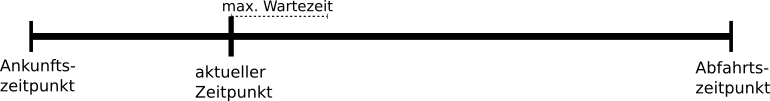
\includegraphics[width = \linewidth]{img/SA_participants_Graph2.png}
	\caption{Beispielansicht eins Ladeservice}
	\label{SAPart:Graph}
\end{figure}

In der Abbildung \ref{SAPart:Graph} wird beispielhaft die Situation eines einzelnen Fahrzeuges deutlich, welches an dem aktuellen Zeitpunkt eine Kollision registriert hat und nun eine Wartezeit berechnet. Die angedeutete maximale Wartezeit umfasst für jeden aktiven Teilnehmer, dessen Nachricht über das Broadcast System empfangen wurde eine Zeiteinheit. Die tatsächliche Wartezeit des Teilnehmers lässt sich allerdings nicht im Vorhinein bestimmen, da diese per Zufall aus einem Intervall heraus ermittelt wird.
\begin{table}[htb]
\centering
\begin{tabular}{|l|l|l|}
\hline
Zeitpunkt & Fahrzeug Nr. & Ladestand (in \%) \\ \hline \hline
10:00     & 1            & 12,6      \\ \hline
11:30     & 2            & 55,3      \\ \hline
          & 3            & 66,8      \\ \hline
15:00     & 1            & 40,7      \\ \hline
          & 2            & 84,1      \\ \hline
          & 3            & 94,2      \\ \hline
\end{tabular}
\caption{Situation von drei verschiedenen Fahrzeugen zu verschiedenen Zeitpunkten}
\label{tab:example1}
\end{table}

In der Tabelle \ref{tab:example1} ist exemplarisch die Situation von drei Fahrzeugen aufgezeigt, welche zu unterschiedlichen Zeiten ankommen und bei der Ankunft über verschiedene Ladestände verfügen. Die Fahrzeuge werden anhand ihrer Nummer in der mittleren Spalte identifiziert. Alle drei Fahrzeuge beginnen den jeweiligen Ladeservice und beginnen so auch Ladevorgänge. In diesem Beispiel tritt um 15:00 am Nachmittag bei allen drei Ladevorgängen eine Kollision auf. Da die Kollision bei allen Teilnehmern auftritt berechnen auch alle Teilnehmer eine Wartezeit. Das Intervall, aus dem diese Wartezeit bestimmt wird, ist für alle Teilnehmer gleich, es lautet [0,3]. Welche Wartezeiten die Teilnehmer tatsächliche abwarten müssen entscheidet allerdings das Ergebnis der Zufallsfunktion.

\subsection{Wartezeit über Teilnehmer und Fahrzeugparameter}
\label{cap:background_sec:SA_waitingTime}
Ähnlich zu dem Vorgehen in Kapitel \ref{cap:background_sec:SA_participants}, bei der Methodik SA+T, wird auch bei diesem Ansatz der in Kapitel \ref{capBody:VDE} vorgestellte Spannungsregler erweitert. Auch bei diesem Ansatz werden lediglich Spannungskollisionen betrachtet und es werden keine aktiven Maßnahmen bei einer zu hohen Last am Transformator ergriffen. Diese Methodik wird im Folgenden mit SA+T+F bezeichnet. Der Unterschied zur Methodik SA+T ist die Art und Weise der Berechnung der Wartezeit. Der Wert der Wartezeit wird auch hier per Zufall aus einem Intervall heraus bestimmt. Der Unterschied liegt in der Art der Bestimmung der oberen Grenze dieses Intervalls. Die obere Grenze wird durch Ausführung einer Formel bestimmt, welche von drei Parametern abhängt.  Der erste Parameter gibt an wie viele Zeiteinheiten, zwischen dem aktuellen Zeitpunkt und dem Zeitpunkt, an dem das Fahrzeug die Ladestation wieder verlässt, liegen. Dieser Parameter wird im Folgenden mit „verbleibende Zeit“ oder t\textsubscript{V} bezeichnet. Der zweite Parameter gibt an, wie viel Zeit noch benötigt wird, um den Akku des Fahrzeuges auf einen Ladestand von 100~\% zu bringen. Für diese Berechnung wird allerdings die Normspannung verwendet und nicht die aktuell gemessene Spannung. Dieser Parameter wird im Folgenden mit „verbleibende Ladezeit“ oder t\textsubscript{L} bezeichnet. Die beiden Parameter, verbleibende Zeit und verbleibende Ladezeit, werden lokal von jedem Teilnehmer für sich selbst bestimmt, sie benötigen dafür keinen weiteren Input. Der dritte Parameter ist die aktuelle Anzahl an Teilnehmenden T. Diese Parameter wurden gewählt mit dem Ziel Fahrzeuge, welche erst weniger geladen habe, oder Fahrzeuge, deren Abfahrt kurz bevorsteht, besserzustellen. Durch den Einfluss der Teilnehmerzahl, wird aber auch die Aktivität im Netz mit in Betracht gezogen. Diese drei Parameter, die verbleibende Zeit t\textsubscript{V}, die verbleibende Ladezeit t\textsubscript{L} und die Anzahl der Teilnehmer T werden in folgende Formel eingesetzt um die obere Grenze G\textsubscript{O}:
\begin{align}
	G\textsubscript{O} = \frac{t\textsubscript{V} - t\textsubscript{L}}{T}
	\label{SA:formel4}
\end{align}
Der Ergebnisbereich der Formel \ref{SA:formel4} ist nach oben durch den Faktor 't\textsubscript{V} - t\textsubscript{L}' begrenzt und nach unten aufgrund der Division des Faktors durch minus unendlich. Das Ergebnis dieser Formel beschränkt nun das Intervall, aus dem die Wartezeit bestimmt wird, nach oben. Die Subtraktion von der verbleibenden Ladezeit und der verbleibenden Zeit, gibt nun an, wie viel Zeit das Fahrzeug neben der, welche zum Laden benötigt wird, noch zusätzlich hat. Diese Zeit würde das Fahrzeug also nicht zum Laden benötigen. Ein Sonderfall tritt auf, wenn das Ergebnis dieser Formel kleiner ist als Eins. Dies kann passieren, wenn etwa die verbleibende Zeit geringer ist als die verbleibende Ladezeit. Tritt dieser Fall ein wird erneut eine obere Grenze für das Intervall bestimmt. Dies ist notwendig, da das Ergebnis der Formel \ref{SA-formel5} die obere Grenze eines Intervalls berechnet, aus welchen eine ganze Zahl gezogen werden soll. Ist die obere Grenze nun aber kleiner als Eins und die untere Grenze ist Null, so gibt es nur eine ganze Zahl in diesem Intervall und die Verwendung der Zufallsfunktion würde keinen Mehrwert bringen. Tritt aber dieser Fall ein muss eine andere Formel verwendet werden. Die Formel, die in diesem Fall verwendet wird, hat nur einen Parameter. Dieser Parameter ist die zuvor berechnete obere Grenze des Intervalls, bezeichnet mit G\textsubscript{alt}. Zur Bestimmung des neuen Wertes wird folgende Formel verwendet \\
\begin{align}
	G\textsubscript{O} = 10 \cdot (1 - e^{G\textsubscript{alt} - 1}) + 1
	\label{SA-formel5}
\end{align}
Der Parameter der Formel \ref{SA-formel5} liegt im Bereich von minus unendlich bis Eins. Die Formel wurde entwickelt mit dem Ziel Werte zwischen Eins und Elf zu liefern, wobei sich eine anfängliche Differenzierung der Ergebnisse bei kleiner werdenden Werten des Parameters einstellen sollte. Das Ergebnis dieser Formel grenzt nun das Intervall, aus dem die Wartezeit bestimmt wird, nach oben ab. Das Verhalten während einer Wartezeit, welche mithilfe dieser Formel \ref{SA-formel5} abgegrenzt wurde, kann sich von dem Verhalten einer Wartezeit welche durch Formel \ref{SA:formel4} abgegrenzt wird unterscheiden. Wenn eine solche Wartezeit das erste Mal bestimmt wird, unterscheidet sich das Verhalten in drei Punkten. Der Erste wäre, dass die Verbindung zum Netz nicht getrennt wird, es wird also weiterhin Leistung aus dem Netz bezogen. Der zweite Unterschied liegt in der Bestimmung der möglichen Ladeleistung, statt mit der Formel \ref{Main_formula3} wird, entgegen dem eigentlich verwendetem Spannungsregler, die Formel \ref{Main_formula1} verwendet. Der dritte Unterschied ist das veränderte Verhalten beim Auftreten von Kollisionen, diese werden nicht beachtet und es wird nicht auf sie reagiert. Eine solche Art der Wartezeit kann allerdings nicht mehrmals direkt hintereinander wahrgenommen werden. Tritt nach Beendigung dieser Wartezeit sofort wieder eine Kollision auf, muss eine normale Wartezeit abgewartet werden, auch wenn das Intervall mithilfe der Formel \ref{SA-formel5} begrenzt wurde. Nach dieser Wartezeit ist eine solche Sonderbehandlung allerdings wieder möglich.\\
\begin{figure}[htb]
	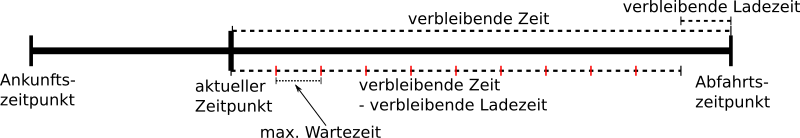
\includegraphics[width = \linewidth]{img/SA_waiting_Graph4.png}
	\caption{Beispielansicht eines Ladeservices}
	\label{SAWait:Graph}
\end{figure}

In der Abbildung \ref{SAWait:Graph} ist eine exemplarische Darstellung einer Situation eines Fahrzeuges deutlich, welche zu diesem aktuellen  Zeitpunkt eine Kollision registriert. Oberhalb sind die beiden Parameter „verbleibende Zeit“ und „verbleibende Ladezeit“ angetragen. Unterhalb verdeutlicht eine gestrichelte Linie das Ergebnis der Subtraktion dieser beiden Werte. Die vertikalen Linien stehen für die Aufteilung nach der Division durch die Anzahl der Teilnehmer. Ebenfalls angezeigt wird die Länge eines dann verblieben Teiles des Ergebnisses der Subtraktion, die Anzahl der Zeiteinheiten eines solchen Restes begrenzt in diesem Fall das Intervall der Wartezeit noch oben.\\
\begin{table}[htb]
\centering
\begin{tabular}{|l|l|l|l|}
\hline
Zeitpunkt & Fahrzeug Nr. & Ladestand & Abfahrtszeitpunkt \\ \hline \hline
10:00     & 1            & 12,6      & 19:00             \\ \hline
11:30     & 2            & 55,3      & 19:00             \\ \hline
          & 3            & 66,8      & 19:00             \\ \hline
15:00     & 1            & 40,7      & 19:00             \\ \hline
          & 2            & 84,1      & 19:00             \\ \hline
          & 3            & 94,2      & 19:00             \\ \hline
\end{tabular}
\caption{Situation von drei verschiedenen Fahrzeugen zu verschiedenen Zeitpunkten}
\label{tab:example2}
\end{table}

In der Tabelle \ref{tab:example2} wird das Beispiel aus Tabelle \ref{tab:example1} aus Kapitel \ref{cap:background_sec:SA_participants} wiederaufgegriffen. Berechnet man nun allerdings die Wartezeit mit der hier vorgestellten Methodik, weichen die Ergebnisse voneinander ab. Für das Fahrzeug mit der Nummer~1 wurde bei einer verbleibenden Zeit von vier Stunden und 40,7\% Ladestand eine maximale Wartezeit von 60 Zeiteinheiten bestimmt. Beim Fahrzeug~2 sollte nun bei selber verbleibender Zeitmenge aber höherem Ladestand auch eine höhere, maximale Wartezeit berechnet werden. Die maximale Wartezeit für das Fahrzeug~2 beträgt 75 Zeiteinheiten, somit tritt ein, was gemäß der abgeänderten Berechnung eintretten soll, die maximale Wartezeit von Fahrzeug~2 ist höher als die von Fahrzeug~1. Die Situation zwischen Fahrzeug~3 und Fahrzeug~2 ist ähnlich zu der zwischen Fahrzeug~1 und 2. Fahrzeug~3 sollte eine höhere maximale Wartezeit aufweisen als Fahrzeug~2 und bei 78 Zeiteinheiten ist dies auch der Fall.  

\section{Slotted ALOHA Spannungsregler mit Transformatorlaststeuerung}
Die Laststeuerung am Transformator soll dazu beitragen die Ausgangsleistung des Transformators im Niederspannungsnetz besser zu regeln und zu limitieren. Die Limitierung der Ausgangsleistung trägt erstens zur Schonung des Transformators an sich bei, aber auch die sich im Stromnetz bewegende Leistung wird limitiert. Die Regelung der möglichen Transformatorlast erfolgt gemäß dem Vorbild des VDE Spannungsregler, bekannt aus dem Kapitel \ref{capBody:VDE}. Die mögliche Ladeleistung wird abhängig von der aktuellen Transformatorlast geregelt. Es wurde ein Limit festgelegt, welches als Obergrenze verwendet wird. In einem Bereich von 80~\% bis 100~\% wird die mögliche Ladeleistung linear reduziert. Bei einer Transformatorlast von weniger als 80~\% steht die mögliche Ladeleistung komplett zur Verfügung. Bei einer Transformatorlast, welche über dem Limit liegt, kann keine Ladeleistung mehr abgerufen werden.  \\
\begin{figure}[htb]
	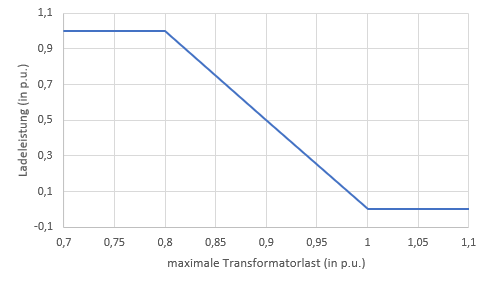
\includegraphics[width = \linewidth]{img/TrafoGraph1.png}
	\caption{Transformatorlast zu Leistungsverhältnis}
	\label{SATrafo:Graph}
\end{figure}

In der Abbildung \ref{SATrafo:Graph} zeigt die mögliche Ladeleistung bei dem prozentualen Anteil der maximalen Transformatorlast. Auf der Y-Achse ist die mögliche Ladeleistung angetragen, wobei die Eins für die höchstmögliche Leistung steht und Null dafür, das keine Leistung abrufbar ist. An der X-Achse werden die aktuell anliegenden Prozent der Normspannung angetragen. An dem Graphen ist ersichtlich wie sich eine ansteigende Transformatorlast auf die mögliche Ladeleistung auswirkt. Ebenso wird im Vergleich mit der Abbildung \ref{Abb_VDEController} ersichtlich, wie die Arbeitsweise der beiden Regler übereinstimmt. Der Faktor gibt an welcher Anteil der Ladeleistung bei der aktuellen Transformatorlast verfügbar ist. Ergebnisse größer als Eins werden auf Eins reduziert, da alle Werte größer als Eins in einer höheren Ladeleistung als möglich resultieren würden. Der Wert des Faktors F\textsubscript{T} wird mit folgender Formel bestimmt \\
\begin{center}
	$ F = \begin{cases}
	1 &  \text{$<$ 80\% maximaler Last} \\
	0 &  \text{$>$100\% maximaler Last} \\
	- \frac{10}{403333} \cdot L\textsubscript{T} + 5 & \text{$>$ 80\%, $<$ 100\% maximaler Last}
	\end{cases}$
\end{center}
Der Wert der aktuellen Transformatorauslastung wird ähnlich zu der Anzahl der Teilnehmer über das Broadcastsystem verteilt. Liegt der Wert nicht vor, wird ein Wert nahe am Limit gewählt, um die Last so niedrig zu halten, aber dennoch noch einen Lastbezug zu zulassen. Der Faktor der Transformatorlast wird ebenso wie der Faktor zur Spannung in der Formel \ref{Main_formula1} berücksichtigt, dadurch verändert sich die Formel \ref{Main_formula3} wie folgt
\begin{align}
	P\textsubscript{L} = U\textsubscript{A} \cdot I\textsubscript{F} \cdot F\textsubscript{S} \cdot F\textsubscript{T} \label{Main_formula4}
\end{align}
Neben der Formel zur Berechnung der möglichen Leistung, wird auch der verwendete Lag-Filter rekonfiguriert. Am Vorgehen bei der Erhöhung der Werte wird nichts verändert, lediglich das Verhalten bei der Verringerung von Werten wird angepasst. Die Gründe für eine Verringerung der Leistung sind eine gesunkene Stromstärke, eine gesunkene Spannung oder ein verändertes Ergebnis der beiden Faktoren für Spannung und Transformatorlast. Das geänderte Verhalten tritt nur auf, wenn eine Transformatorkollision vorliegt, da eine Kollision einen laufenden Ladevorgang beendet, fällt nach einer Kollision immer der Wert der bezogenen Leistung. Tritt eine Transformatorkollision auf, ergibt die Formel \ref{Main_formula4} immer 0. Der in Kapitel \ref{capBody:VDE} eingeführte Filter würde 63,2~\% der nötigen Änderung vornehmen, der hier vorgestellte Filter nimmt jedoch nur 36,8~\% der Änderung vor. Der gewählte Wert ist der Kehrwert von 63,2~\%, 100~\% - 63,2~\% = 38,2~\%. Die Veränderung am Lag-Filter wurde vorgenommen, da aller Teilnehmer von einer Transformatorkollision betroffen sind, und so auch alle Teilnehmer nach einer Transformatorkollison die bezogene Leistung reduzieren müssen. Aufgrund geringeren Abnahme pro Teilnehmer pro Zeitschritt, sinkt die Transformatorlast langsamer ab. Dieses langsamere Absinken beugt bei hohen Teilnehmerzahlen einem zu großem Einbruch an Transformatorlast vor und führt so besseren Verteilung der Abnahme. Tritt eine Spannungskollision auf sinkt die bezogene Leistung weiterhin mit der unveränderten Rate von 63,2~\% ab, dies ist auch der Fall tritt eine Transformatorkollision und eine Spannungskollision bei einem Teilnehmer gleichzeitig auf. Bei einer Spannungskollision bleibt das Verhalten unverändert, da der Zusammenhang zwischen zu hohem Leistungsbezug und Spannungsabfall weniger direkt in Verbindung steht, wie bezogene Leistung und Transformatorlast. 
\begin{figure}[htb]
	\centering
	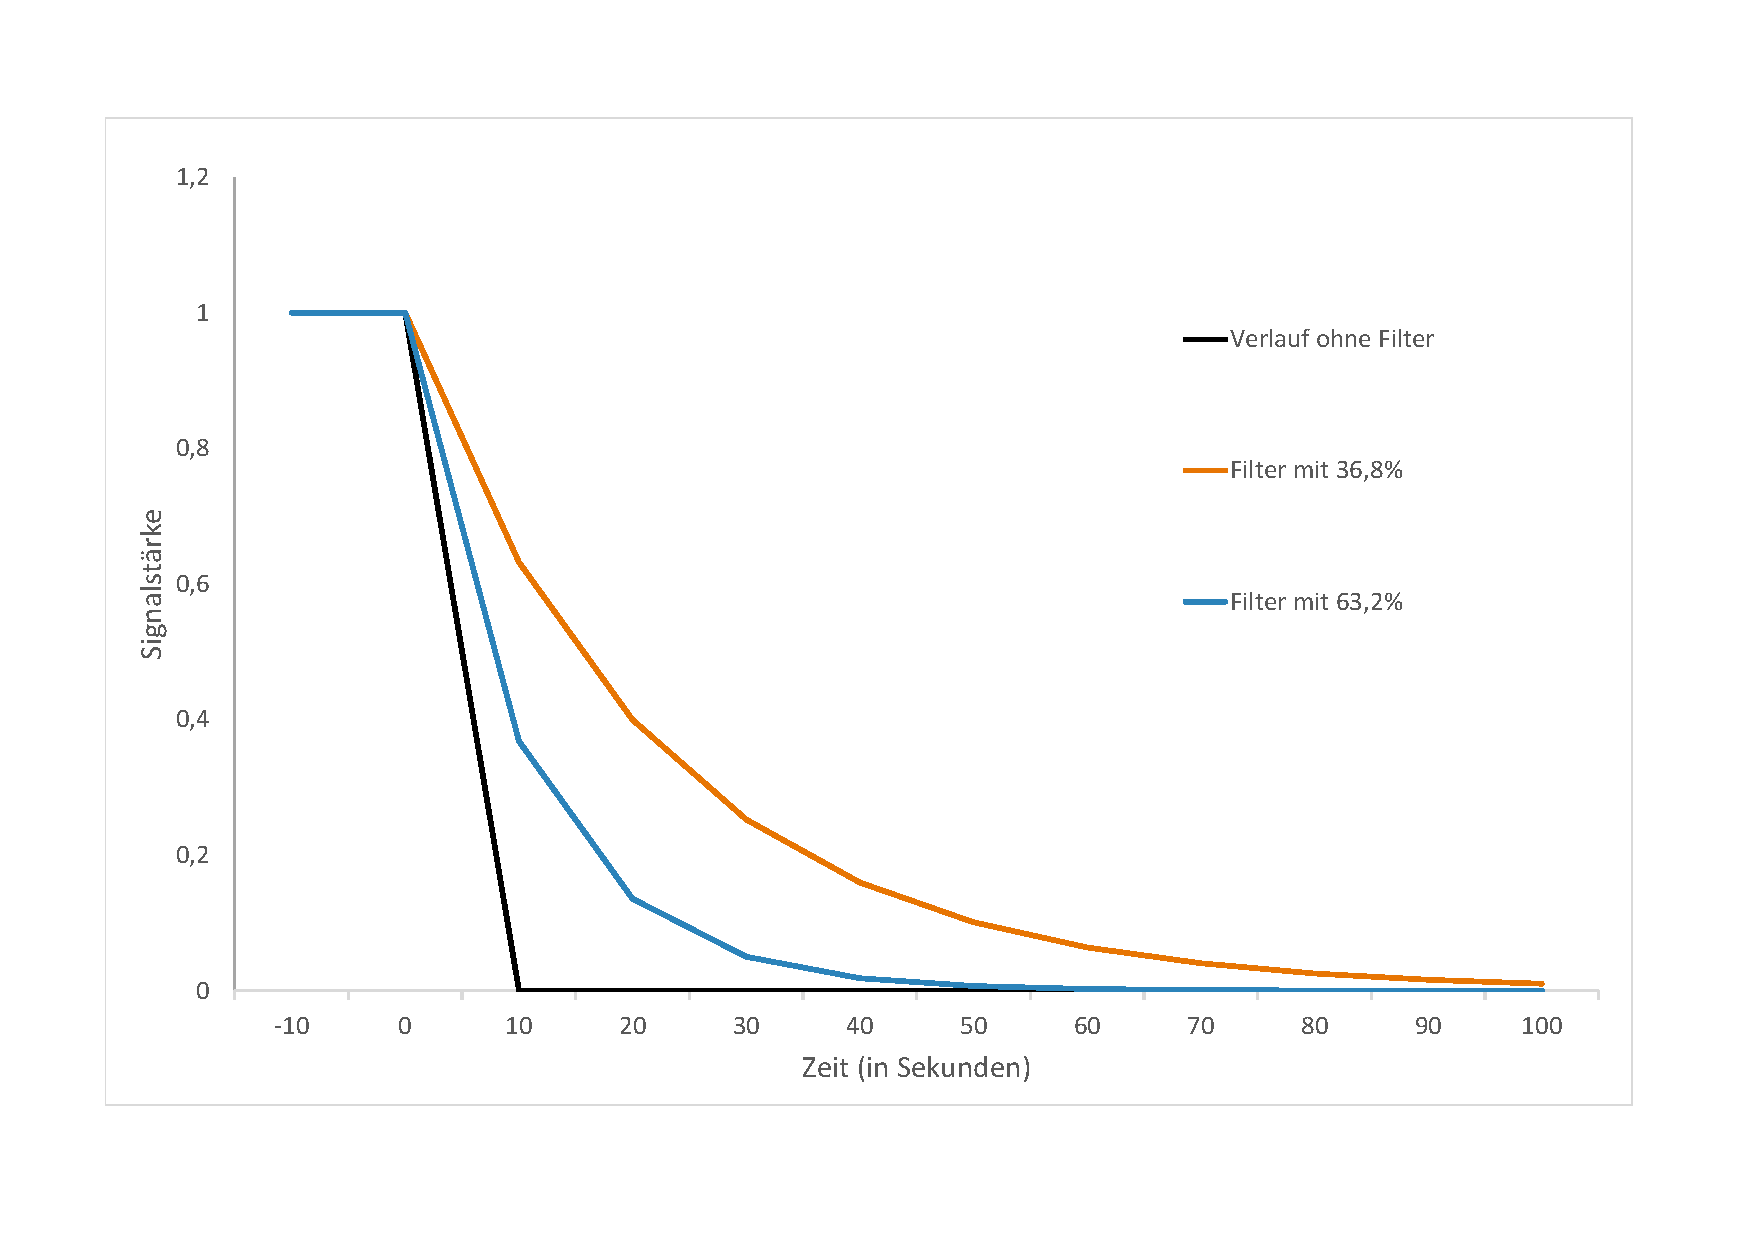
\includegraphics[scale=0.4]{img/lag_Filter6.pdf}
	\caption{Wirkung eines First-Order Lag Filters beim Wechsel des \newline Eingangsignals von 0 auf 1 bei verschieden starker Filterung}
	\label{SATrafo:lagFilter}
\end{figure}

In Abbildung \ref{SATrafo:lagFilter} wird die Auswirkung der verschiedenen Filter dargestellt. Die Abnahme bei einem Filter mit 36,8~\% dauert etwa doppelt so lange wie wenn ein Filter mit 63,2~\% verwendet werden würde. Die beiden Kurven der verschiedenen Filter haben aber dennoch die selbe grundlegende Form.\\
Die bisher bekannten Methodiken VDE, SA+T und SA+T+F sind alle um den Transformatorkontroller erweiterbar, nach der Erweiterung werden sie mit VDE+Tr, SA+T+Tr und SA+T+F+Tr bezeichnet.
